% !TeX root = ../Aquila_Pflichtenheft.tex

\chapter{Projektplanung} \label{chapter:projektplanung}
\section{Projektstrukturplan}

{\centering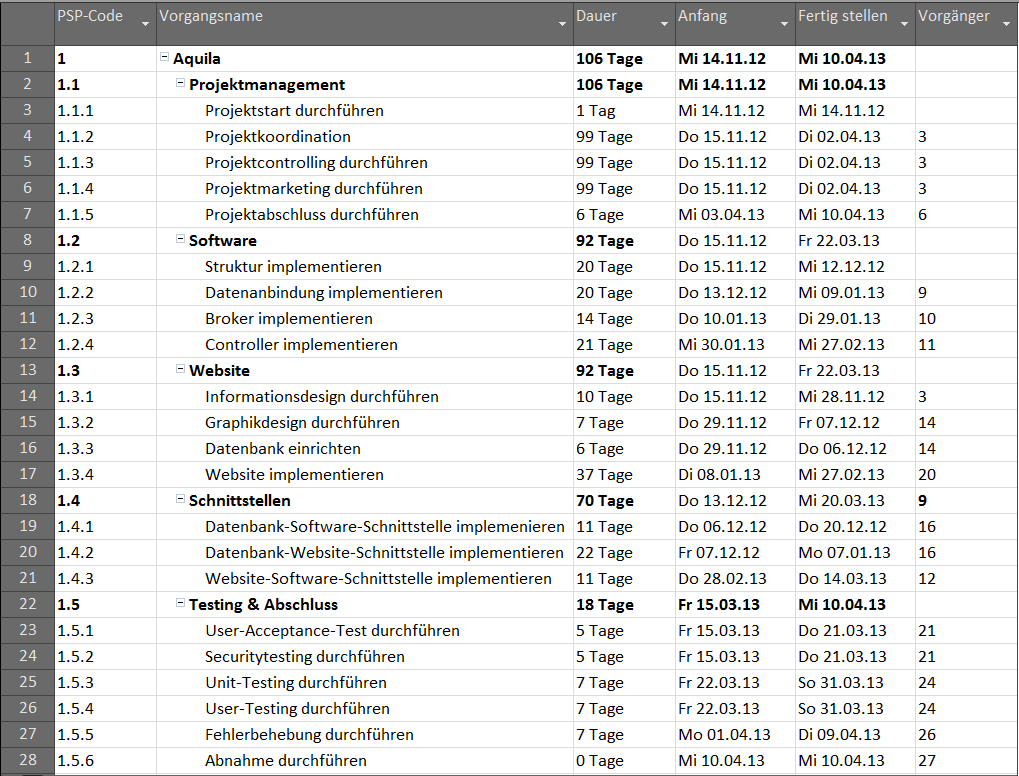
\includegraphics[width=1.00\textwidth]{graphics/projektplanung/psp.png}
\captionof{figure}{Projektstrukturplan}}

\section{Balkenplan}

{\centering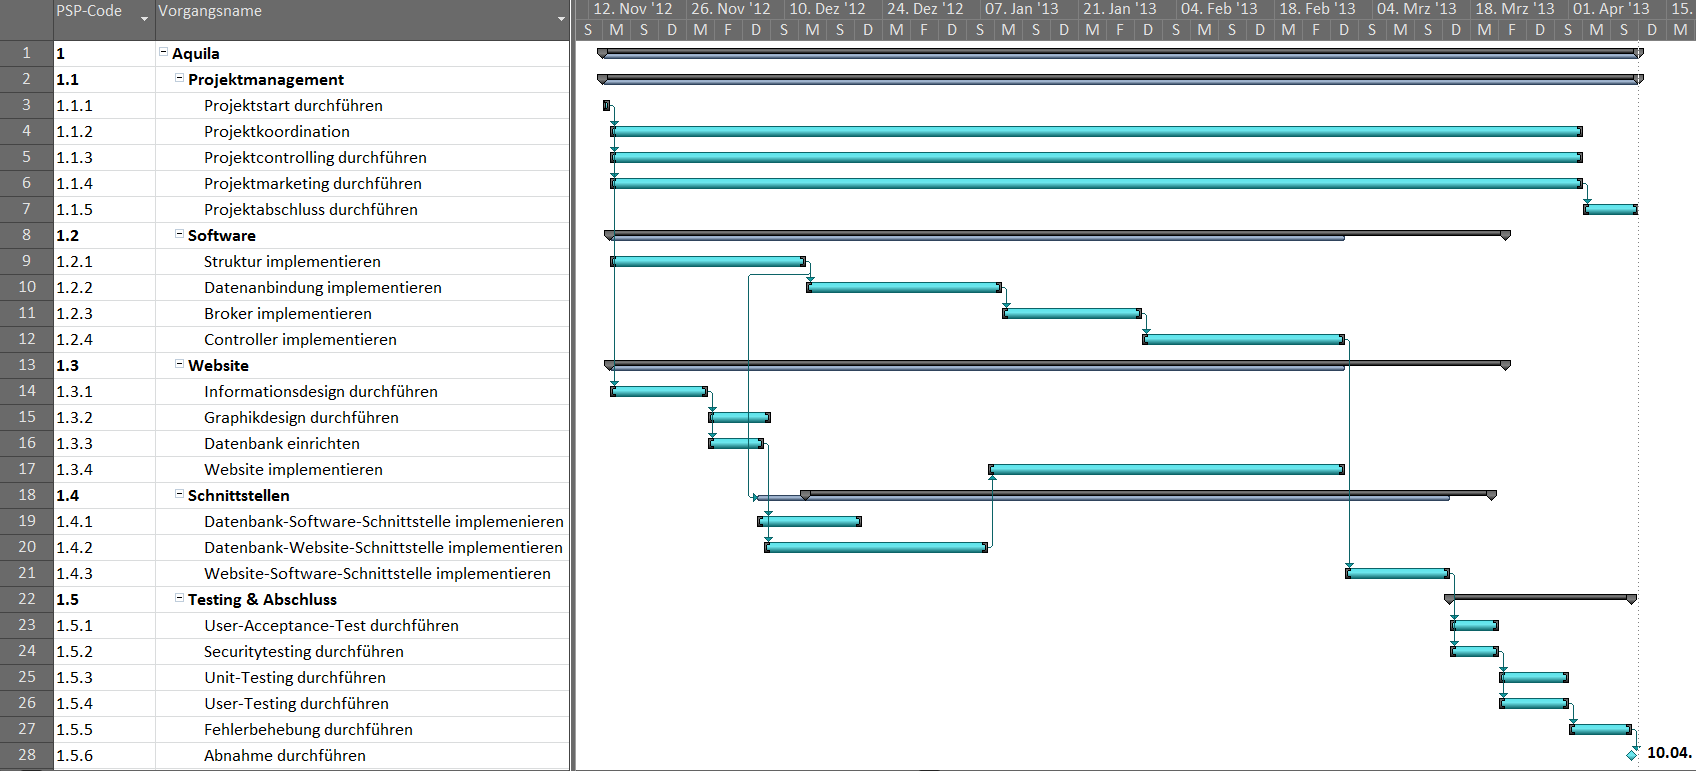
\includegraphics[width=1.00\textwidth]{graphics/projektplanung/balkenplan.png}
\captionof{figure}{Balkenplan}}

\section{Meilensteinplan}

\begin{center}

\begin{tabular}{ | p{3.5cm} | p{7.5cm} | l |}
\hline 
\textbf{Meilenstein} & \textbf{Deliverable} & \textbf{Datum}\\  \hline
Projektstart & ~ & 14.11.2012 \\  \hline
Datenbank eingerichtet & Script zum Erstellen der Datenbank + dazugeh�rige Dokumentation & 06.12.2012 \\ \hline
Externe Schnittstellen implementiert & Schnittstellen zur Kommunikation mit eSignal und InteractiveBrokers + dazugeh�rige Dokumentation & 29.01.2013 \\ \hline
Software \& Website fertiggestellt & Tradingsoftware mit simplem Algorithmus und Websiteoberfl�che und Charting + dazugeh�rige Dokumentation & 27.02.2013 \\ \hline
Produkt fertiggestellt & Version des Produkts (inklusive aller internen Schnittstellen), die noch nicht getestet wurde + dazugeh�rige Dokumentation & 14.03.2013 \\ \hline
Testing abgeschlossen & Testberichte und etwaige Verbesserungen am Produkt & 09.04.2013 \\ \hline
Projektabnahme & Ausgef�lltes Abnahmeprotokoll & 10.04.2013 \\ \hline

\end{tabular}

\end{center}